\documentclass[12pt]{article}
\usepackage[letterpaper, portrait, margin=1in]{geometry}
\usepackage[hidelinks]{hyperref}
\usepackage{setspace}
\usepackage{fancyhdr}
\usepackage{graphicx}
\usepackage[T1]{fontenc}
\usepackage{mathptmx}
\usepackage[backend=biber, style=mla]{biblatex}
\pagestyle{fancy}
\addbibresource{proposal.bib}    
\fancyhf{} % sets both header and footer to nothing}
\renewcommand{\headrulewidth}{0pt}
\pagenumbering{arabic}
\rhead{Sheehan \thepage} 
\fancypagestyle{1stPage}{
    \fancyhf{}
    \renewcommand{\headrulewidth}{0pt} % removes horizontal header line
    \lhead{Owen M. Sheehan \\ Tina Cafasso \\ Interpretation and Argument \\ 12/14/23}
    \rhead{ Sheehan 1}
}

\thispagestyle{1stPage}
\begin{document}
\begin{doublespace}
    \vspace*{20pt}
% #region Abstract
\section*{Abstract}
    \par As the Internet gets older, the way we perceive authenticity changes, there is little research into how we interact with each other in the last year or so.
        As the generation that grew up on the Internet gets older, the levels of cynicism regarding authenticity gets higher.
        This is due to a change in how we use social media, when it started, social media was for sharing short candid stories about ones life or work.
        However, in the modern world, the attitude has shifted toward presenting a sculpted image of ones self. 
        This has led to increased levels of skepticism as people are more cognizant of the fact that a lot of social media posts serve to make people look better.
% #endregion

\newpage
% #region Intro
    \section*{Introduction}
    \par This essay will look at the current research regarding authenticity online and then propose research on how the average person perceives authenticity online.
        To begin, we will look at the current research consensus and look on how it can be expanded.
        Previous research has been done on how people interact with authenticity online, however, most of these articles get their data from systematic reviews of certain peoples accounts online,
        while others instead ask participants via social media about their thoughts on social media.
        I believe that this can be a flawed way to go about getting data for such studies as it is reliant on people who participate in social media, which may omit some more cynical views of social media.
        As such, I'm going to try and answer the question ``How does the average person perceive authenticity online, do they truly believe what they see, or is it viewed as a facsimile of authenticity''.
% #endregion 

% #region synthesis
\section*{Sythesis}
    \par There are a few concepts that are quite important when talking about authenticity online.
        Firstly, there is the idea of ``Context Collapse'', which is when multiple different audiences get flattened into one \autocite[122]{MB1}.
        Secondly, there is the idea of the ``lowest common denominator'', which is a term created by Bernie Hogan which is the idea that one posts content online that is socially suitable to the people who may not be the intended audience of a post, but can still see the post. \Autocite*[383]{Hogan1}
        These two ideas form the basis for how we look at people's posting behaviours online. It must also be noted that there are a few distinct types of accounts that you will see online, those being personal, professional, and corporate. This essay looks at how people interact with the first two for the most part, as when it comes to authenticity online, corporate accounts don't really matter as most of what they post is marketing materials or ads.
    \par Bernie Hogan uses Erving Goffman's dramaturgical approach, which he describes as ``a metaphorical technique used to explain how an individual presents an ``idealized'' rather than authentic version of herself. 
        The metaphor considers life as a stage for activity. Individuals thus engage in performances, which Goffman defines as ``activity of an individual which occurs during a period marked by his continuous presence before a particular set of observers and which has some influence on the observers''\autocite[22]{Goffman}.
        This continued presence allows individuals to tweak their behavior and selectively \dots \ give off details, a process he termed `impression management.'''\autocite[378]{Hogan1}
        to show that a person's ``performance'' online is catered to an audience that is causing said person's performance to ``consist of the selective details that one presents in order to foster the desired impression alongside the unintentional details that are given off as part of the performance'' \autocite[378]{Hogan1}.
        However, as pointed out by Pitcan et al, social media complicates this as the different ways we present ourselves to separate audiences, or ``code switching'', isn't easily done since the separate audiences are collapsed together. On top of that, the impression management literature based off Goffman, fails to adequately account for the structural differences that affect individuals options and risks. \autocite*[164]{Pitcan1}
    \par To get more information as to how the average person uses self-branding, we can use research done about how microcelebrities use self-branding and extrapolate that to everybody else.
        In Chapter 3 of Alice Marwick's \textit{Status update: Celebrity, publicity, and branding in the social media age}, micro-celebrity is defined as being, ``a state of being famous to a niche group of people, but it is also a behavior: the presentation of oneself as a celebrity regardless of who is pating attention'' \autocite*[114]{Marwick1}.
        One way to achieve this presentation is through self-branding, which in the following chapter Marwick describes as being ``primarily a series of marketing strategies applied to the individual. It is a set of practices and a mindset, a way of thinking about the self as a salable commodity that can tempt a potential employer'' \autocite*[166]{Marwick2}.
        In \textit{`Meat, Mask, Burden': Probing the contours of the branded `self'}, Alison Hearn points out that creating a brand image requires ``creating a detachable, saleable image or narrative, which effectively circulates cultural meaning'' \autocite*[198]{Hearn1}.
        As opposed to self-branding in the real world, the internet ``idealizes transparency ... [and] expect(s) [microcelebrities] to be more available and more ``real'' than stars of the screen or stage'' \autocite[114]{Marwick1}.
    \par To satisfy this expectation, microcelebrities ``creat[e] a persona, produc[e] content, and strategically appeal to online fans by being ``authentic'' '' \autocite[114]{Marwick1}.
        This persona of authenticity, can actually be quite contentious as authenticity is a subjective word, especially when it comes to online audiences, ``Of course, Authenticity is a social construct ... we are interested not in an absolute sense of authenticity, but in what Twitter ... considers `authentic' '' \autocite[119]{MB1}.
        Authenticity on the internet usually takes 2 forms, either direct interaction with ``fans'', or through the sharing of personal information \autocite[114]{Marwick1}.
    \par This creates a schism however, as ``revealing personal information is seen as a marker of authenticity, but is strategically managed and limited'' \autocite[127]{MB1}.
        This becomes a tricky balancing act as that management ``can be seen as \textit{inauthentic}. When asked to describe `authenticity' on Twitter, respondents lpaced it in direct opposition to strategic self-promotion'' \autocite[127]{MB1}.
        Reading all of this, I wanted to see if this skepticism applied not only to micro-celebrities, but also the average person, hence the question ``How does the average person perceive authenticity online, do they truly believe what they see, or is it viewed as a facsimile of authenticity''.
% #endregion 

% #region method 
\section*{Methodology   }
    \par To answer this question, I will be using a survey to gauge people's answers to how they interact with authenticity online, as well as finding out what they consider ``authentic''.
        Questions will include: what social media they use, what kind of accounts they follow, If they think professional or personal accounts are authentic and why, as well as what they consider authentic.
        \underline{\href{https://forms.gle/sjiDcxBzhiiDFehy5}{Link to survery}}.
% #endregion

% #region results
    \newpage
    \section*{Results}
    \begin{figure}[h]
        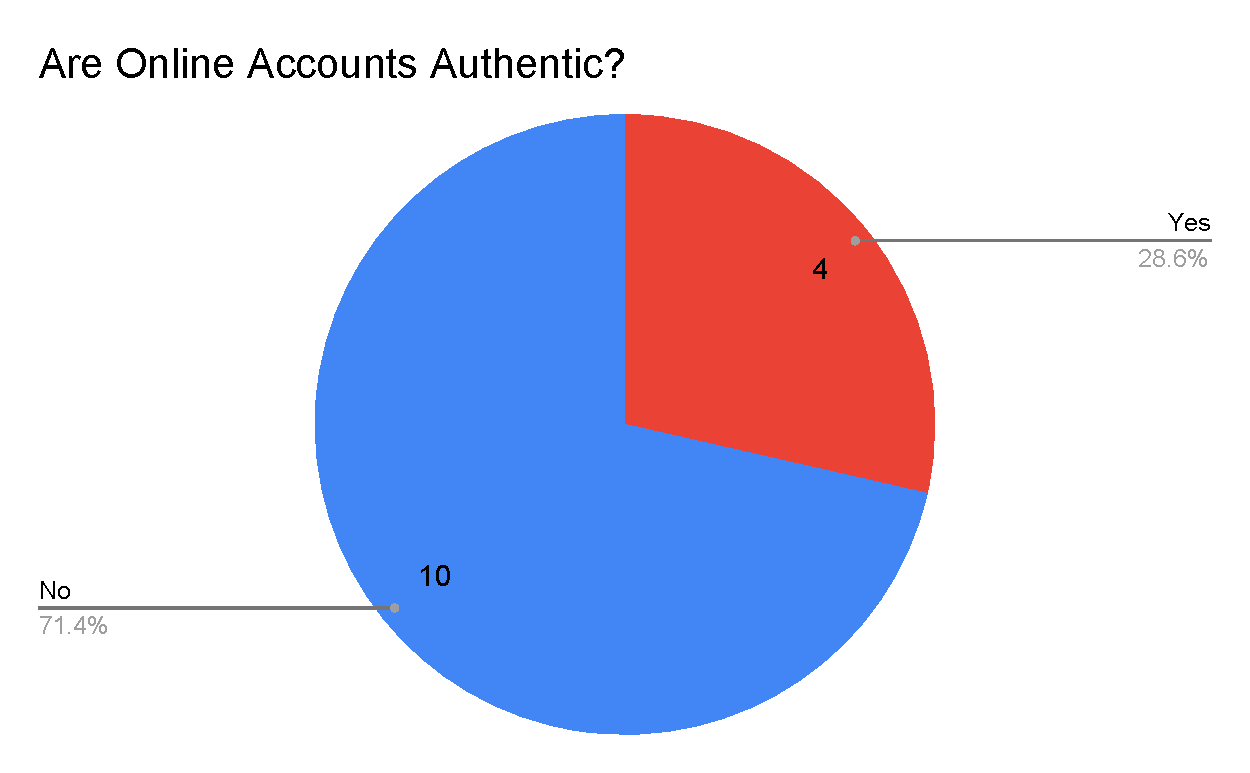
\includegraphics[width=.7\textwidth]{Are Online Accounts Authentic_.pdf}
        \centering
        \caption{Opinions on if online accounts are authentic as a whole.}
        \label{fig:pie1}
    \end{figure}

    \par The main data for my results is seen above in \underline{\hyperref[fig:pie1]{Figure 1}}
        It is worth noting that Figure 1 is an aggregate from questions asking about the authenticity of both personal and professional accounts. See the \underline{\hyperref[sec:appendix]{Appendix}} for the charts relating to those questions.
        What is immediately clear is that, as a whole, respondents believed that online accounts did not post authentic content (\underline{\hyperref[fig:chart2]{Figure 2}}).
    \par When asked about professional accounts, i.e. celebrities, influencers, businesses, respondents almost unanimously stated that these accounts were not authentic. 
        The exception is one response that was yes, however there was no reason given for the answer, making it hard to draw any conclusions from said response.
        The most common reason given as to why professional accounts were not authentic, was, to some extent, ``So much of it is curated and made by a team to serve a purpose'' with that purpose being to ``make money''.
    \par However, when it comes to personal accounts, the proportion of people who thought posts were authentic was only slightly smaller than those who believed that the posts were not. (\underline{\hyperref[fig:chart3]{Figure 3}})
        This result is not surprising, however, some of the reasons given for some responses are.
        Take for example respondent \#5, who believes that authenticity online is showing a completely nuanced view into someones life, ``[Authenticity is] an accurate, portrayal of the subject matter. In the case of social media, the accurate and complete portrayal of ones self and their life. Posts that showcase nuance and normalcy, not just the highlights.''
    \par It must be pointed out that the number of responses collected is no where near large enough to draw any significant conclusions from.
% #endregion 

% #region Conclusion
\section*{Conclusion}
    \par All in all, the results of this ``research'' is not very significant, as stated before there just isn't enough data points to suggest a solid conclusion.
        However, with what little sample size we have, the evidence does seem to suggest that people are as cyncical about their friends authenticity as they are for celebrities. 
        This extrapolation supports a lot of the work of Marwick and boyd, whos work suggest that social media is used mostly as a tool today, which is antithetical to what social media is supposed to be, a place for people to share their thoughts.
    \par Ideally, the results gathered by this research would be more diverse and have more statistical significance, however, we work with what we're given. 
        Anecdotely, most of the people I have spoken to outside of this research also agree that most people aren't authentic online (at least to said persons definition of authentic).
        While that can't really support my conclusion, it does make sense that the generation that grew up with the internet would be more cynical.
    \par When it comes to research focusing on user behavior online, a lot of the articles we looked at focused on the internet in the 2000's and 2010's. This can be quite a bad thing as the relevence of information regarding social media doesn't stay for long, as the ways we interact online change quite rapidly. 



% #endregion

% #region end

    \newpage
    \section*{Appendix}
    \label{sec:appendix}
    \begin{figure}[h]
        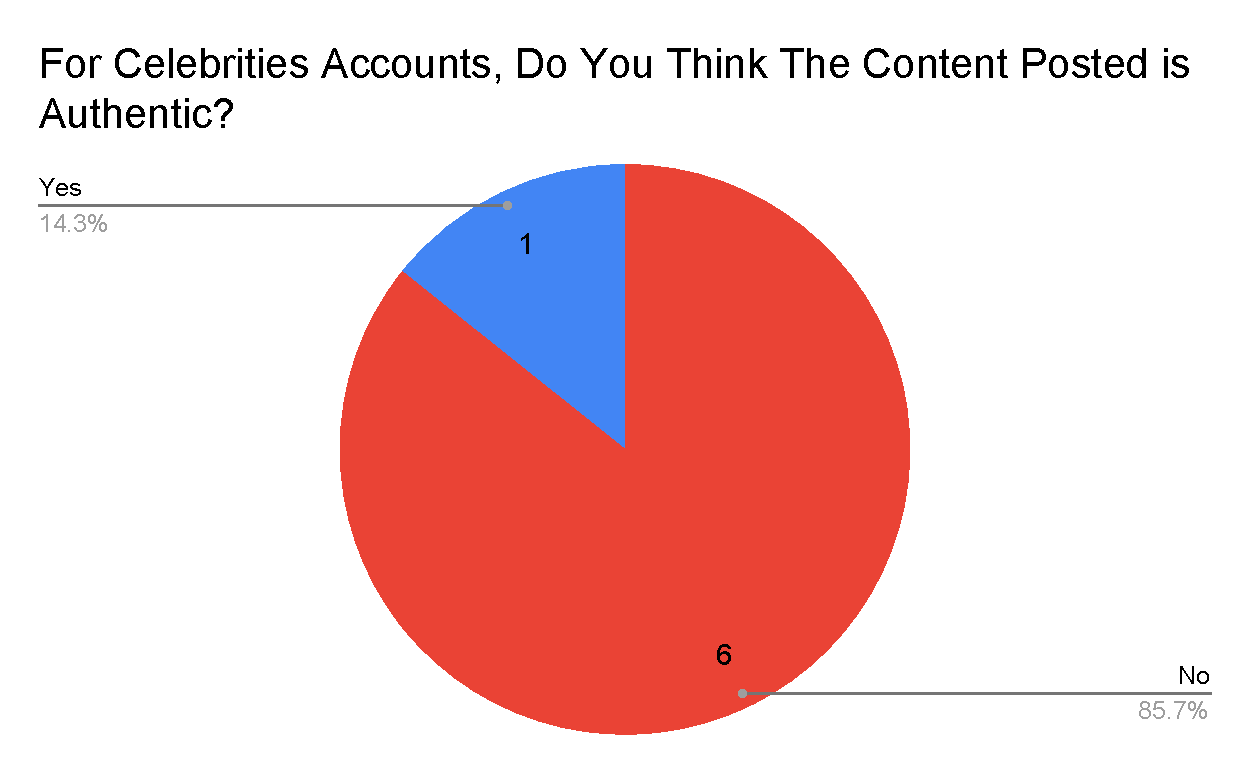
\includegraphics[width=0.7\textwidth]{For Celebrities Accounts, Do You Think The Content Posted is Authentic_.pdf}
        \centering
        \caption{Opinions on the Authenticity of professional accounts}
        \label{fig:chart2}
    \end{figure}

    \begin{figure}[h]
        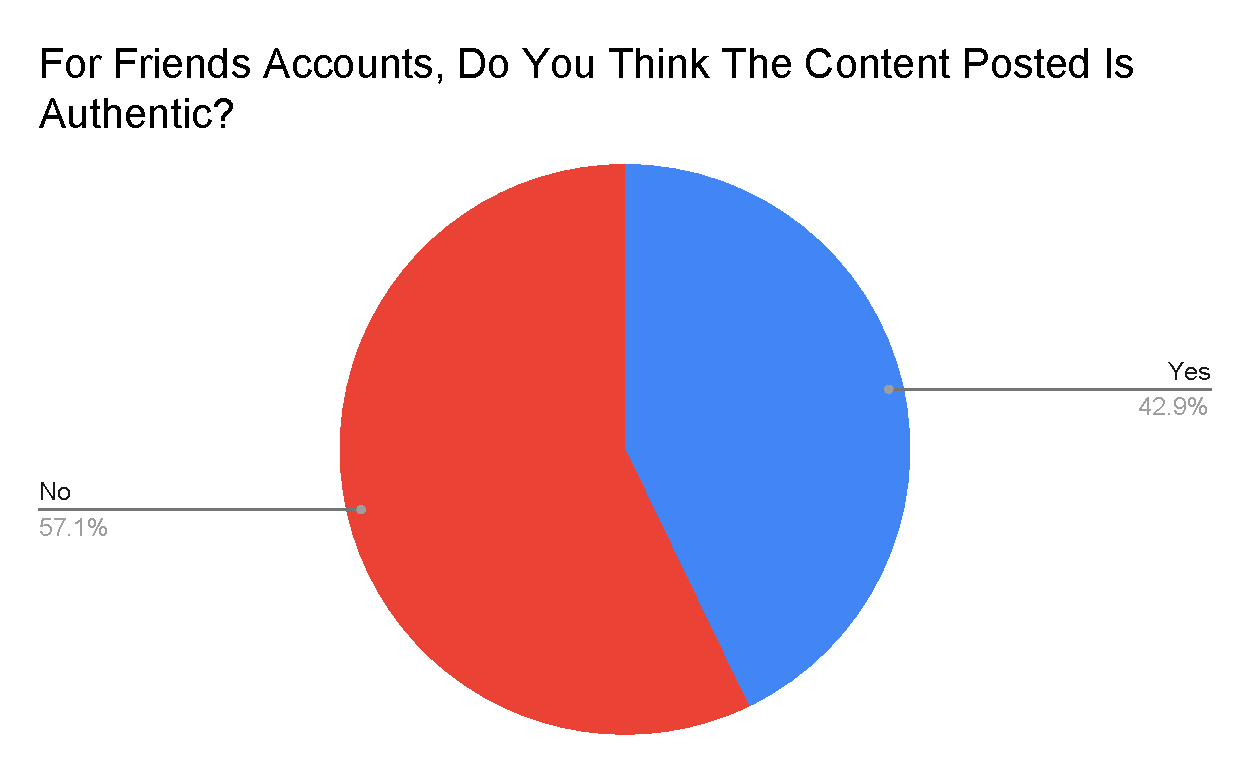
\includegraphics[width=0.7\textwidth]{For Friends Accounts, Do You Think The Content Posted Is Authentic_.pdf}
        \centering
        \caption{Opinions on the Authenticity of personal accounts}
        \label{fig:chart3}
    \end{figure}
% #endregion
\end{doublespace}
\end{document}
